%% DeepCardio-RAG Architecture Diagram — TikZ/LaTeX
%% ====================================================
%% Compile with: pdflatex DeepCardio_RAG_Architecture_TikZ.tex
%% Requires packages: tikz, xcolor, geometry
%%
%% Architecture: 3-Stage Pipeline
%%   Stage 1: ResNet-34 1D-CNN ECG Encoder
%%   Stage 2: Production Milvus Semantic Retrieval (10.228.1.9:19530)
%%   Stage 3: RAG Multi-Head Attention + MoE Classifier + GPT-2 Report Generator

\documentclass[border=10pt]{standalone}
\usepackage{tikz}
\usepackage{xcolor}
\usetikzlibrary{
  shapes.geometric,
  shapes.misc,
  arrows.meta,
  positioning,
  fit,
  backgrounds,
  calc,
  decorations.pathreplacing
}

% ── Color Definitions ────────────────────────────────────────────────────────
\definecolor{stageBlue}{RGB}{59,130,246}        % Stage 1 header
\definecolor{stagePurple}{RGB}{139,92,246}       % Stage 2 header
\definecolor{stageGreen}{RGB}{34,197,94}         % Stage 3 header

\definecolor{bgBlue}{RGB}{219,228,255}           % Stage 1 zone
\definecolor{bgPurple}{RGB}{229,219,255}         % Stage 2 zone
\definecolor{bgGreen}{RGB}{211,249,216}          % Stage 3 zone

\definecolor{nodeBlue}{RGB}{165,216,255}         % Input node
\definecolor{nodePurple}{RGB}{208,191,255}       % ResNet blocks
\definecolor{nodeTeal}{RGB}{195,250,232}         % GAP/projection
\definecolor{nodeGreen}{RGB}{178,242,187}        % Output nodes
\definecolor{nodeOrange}{RGB}{255,216,168}       % Milvus/MoE
\definecolor{nodeYellow}{RGB}{255,243,191}       % Sentence-BERT
\definecolor{nodePink}{RGB}{238,190,250}         % Retriever
\definecolor{nodeRed}{RGB}{255,201,201}          % Coverage loss

% ── TikZ Styles ──────────────────────────────────────────────────────────────
\tikzset{
  %% Stage zones (background rectangles)
  stage zone/.style={
    rectangle, rounded corners=8pt,
    draw, very thick,
    minimum width=#1,
    fill opacity=0.25, draw opacity=0.9,
    inner sep=8pt
  },
  %% Standard node box
  node box/.style={
    rectangle, rounded corners=5pt,
    draw, thick,
    minimum width=4.8cm, minimum height=0.95cm,
    font=\small\sffamily, align=center,
    inner sep=4pt
  },
  %% Emphasized output node
  output box/.style={
    node box,
    draw=stageGreen, line width=2pt,
    fill=nodeGreen
  },
  %% Milvus special box (wider)
  milvus box/.style={
    rectangle, rounded corners=6pt,
    draw=orange!80!black, line width=2pt,
    minimum width=5.5cm, minimum height=2.2cm,
    font=\small\sffamily, align=center,
    fill=nodeOrange, inner sep=6pt
  },
  %% Arrow styles
  main arrow/.style={
    -{Latex[length=8pt,width=5pt]},
    thick, draw=#1
  },
  label arrow/.style={
    main arrow=#1,
    font=\tiny\sffamily
  },
  %% Section header text
  zone title/.style={
    font=\normalsize\bfseries\sffamily, #1
  }
}

% ══════════════════════════════════════════════════════════════════════════════
\begin{document}
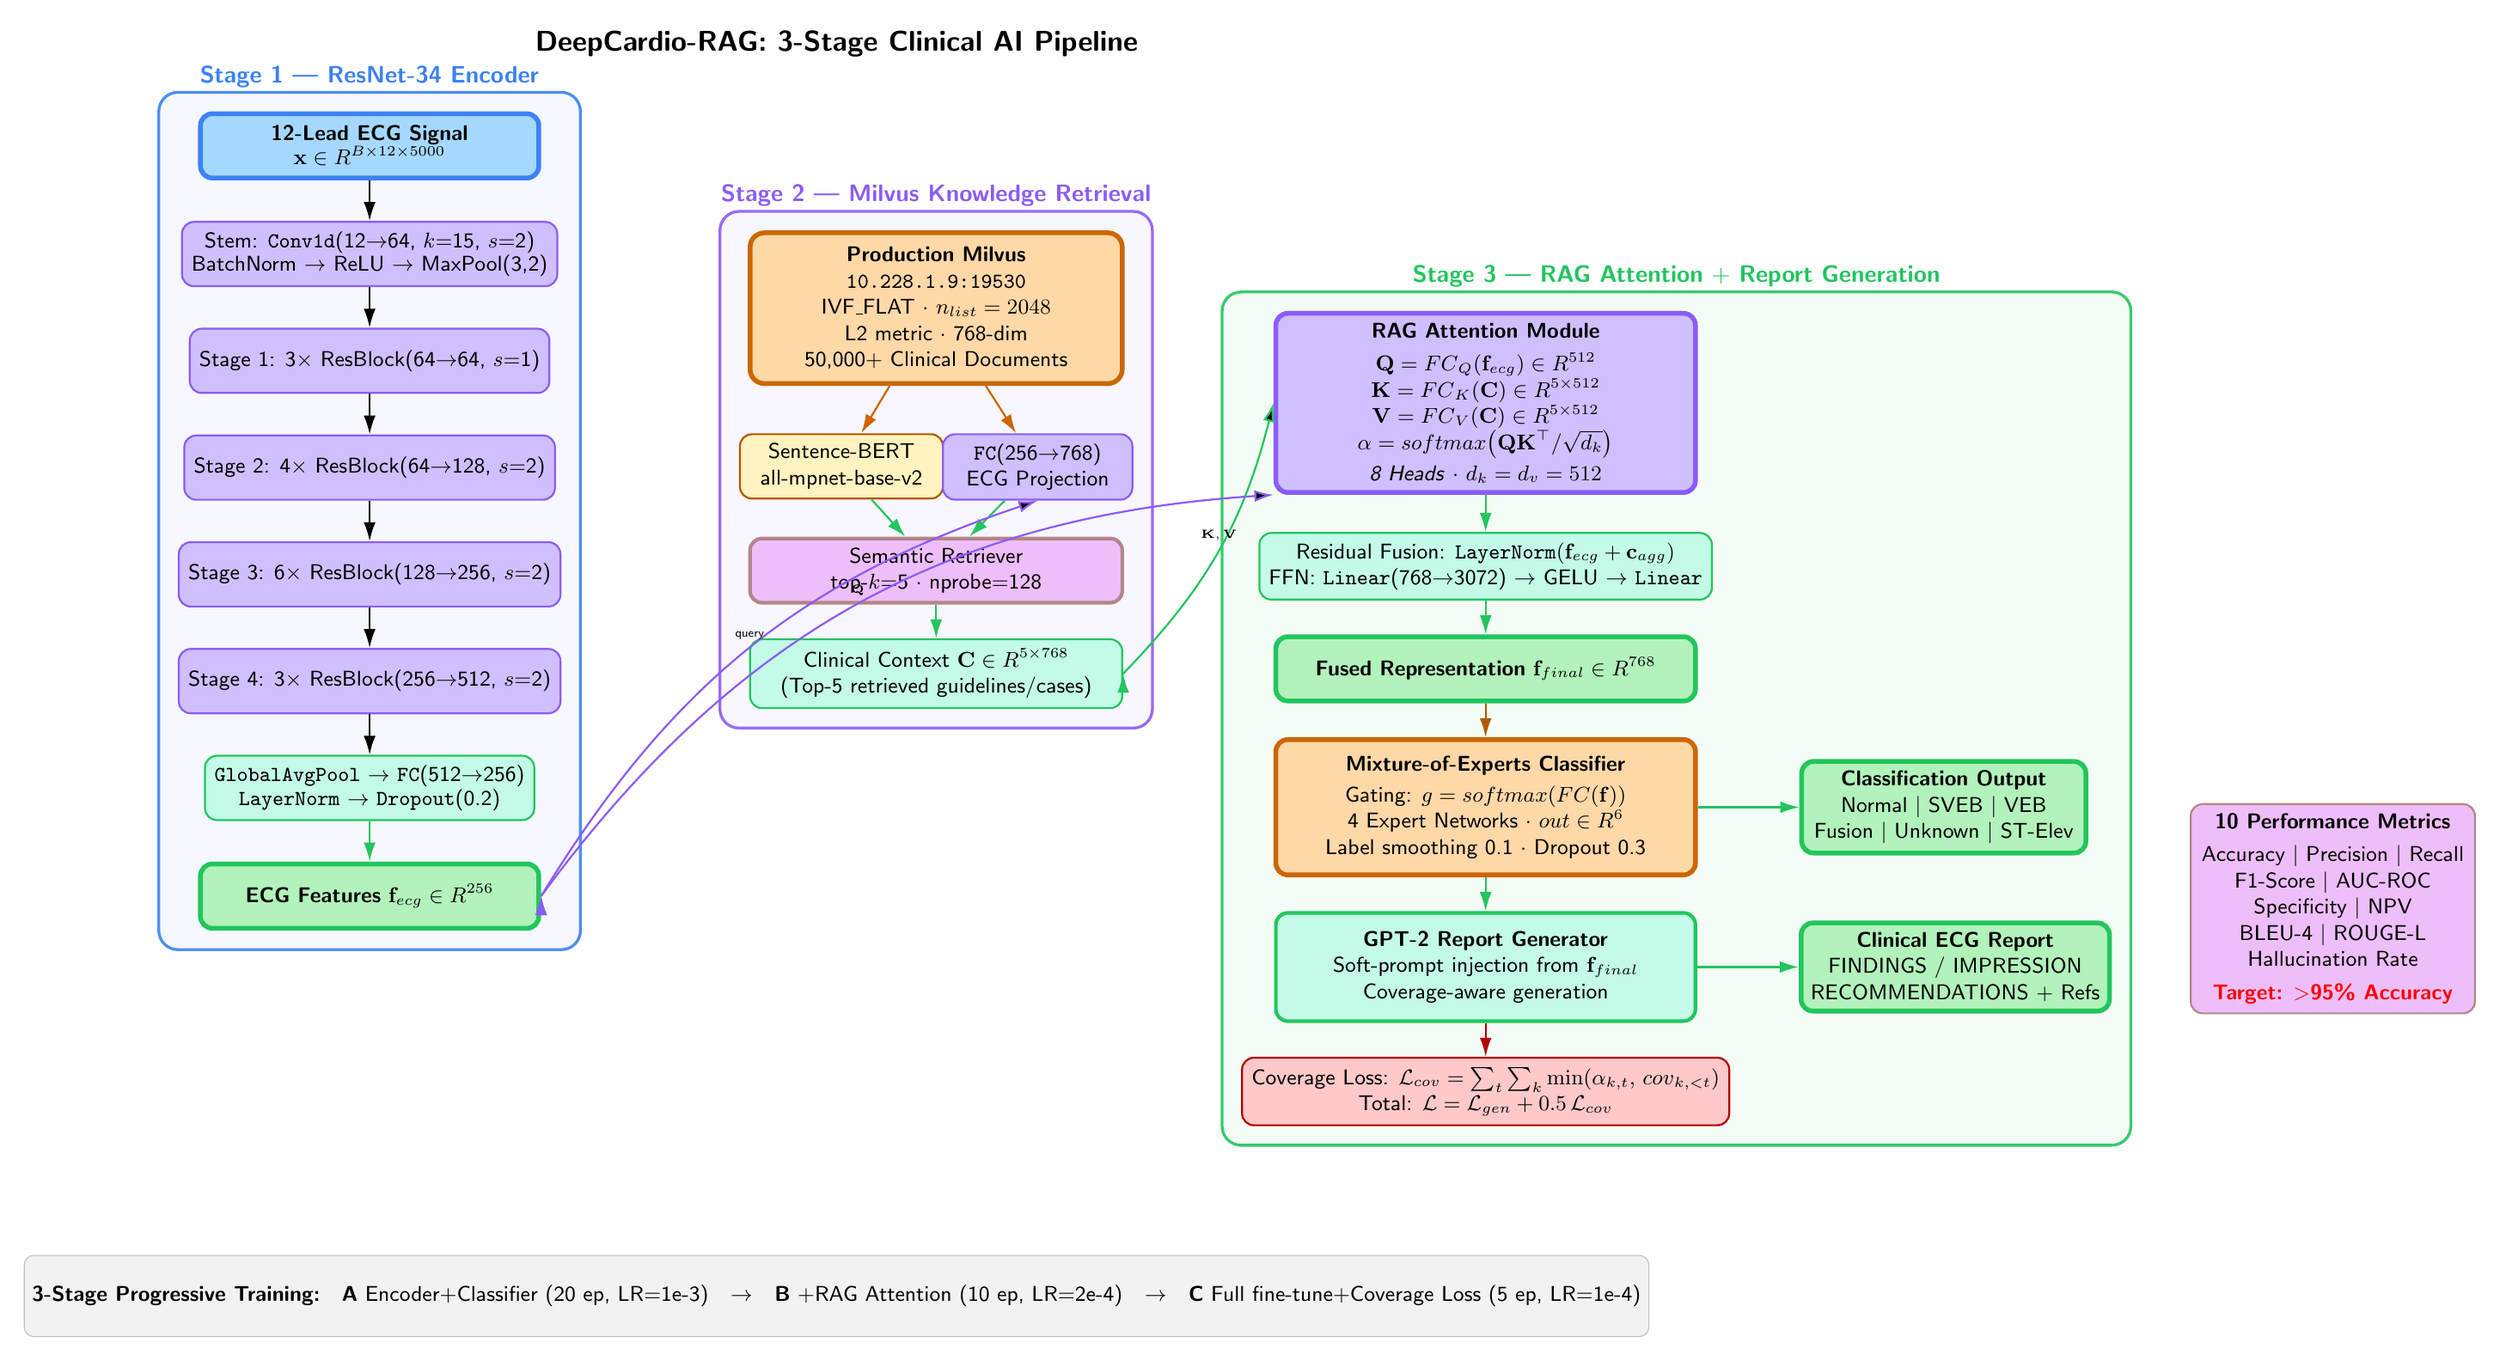
\begin{tikzpicture}[node distance=0.6cm and 1.8cm, >=Latex]

% ── Title ────────────────────────────────────────────────────────────────────
\node[font=\large\bfseries\sffamily, align=center] (title) at (9.5, 1.0)
  {DeepCardio-RAG: 3-Stage Clinical AI Pipeline};

% ══════════════════════════════════════════════════════════════════════════════
% STAGE 1: ResNet-34 ECG Encoder
% ══════════════════════════════════════════════════════════════════════════════

%% Input ECG
\node[node box, fill=nodeBlue, draw=stageBlue, line width=2pt,
      minimum width=5cm]
  (ecg_in) at (2.6, -0.5)
  {\textbf{12-Lead ECG Signal}\\[-1pt] $\mathbf{x} \in \mathbb{R}^{B \times 12 \times 5000}$};

%% Stem block
\node[node box, fill=nodePurple, draw=stagePurple, below=of ecg_in]
  (stem)
  {Stem: \texttt{Conv1d}(12$\to$64, $k$=15, $s$=2)\\[-1pt]
   BatchNorm $\to$ ReLU $\to$ MaxPool(3,2)};

\draw[main arrow=black] (ecg_in) -- (stem);

%% Residual stages
\node[node box, fill=nodePurple, draw=stagePurple, below=of stem]
  (r1) {Stage 1: 3$\times$ ResBlock(64$\to$64, $s$=1)};

\draw[main arrow=black] (stem) -- (r1);

\node[node box, fill=nodePurple, draw=stagePurple, below=of r1]
  (r2) {Stage 2: 4$\times$ ResBlock(64$\to$128, $s$=2)};

\draw[main arrow=black] (r1) -- (r2);

\node[node box, fill=nodePurple, draw=stagePurple, below=of r2]
  (r3) {Stage 3: 6$\times$ ResBlock(128$\to$256, $s$=2)};

\draw[main arrow=black] (r2) -- (r3);

\node[node box, fill=nodePurple, draw=stagePurple, below=of r3]
  (r4) {Stage 4: 3$\times$ ResBlock(256$\to$512, $s$=2)};

\draw[main arrow=black] (r3) -- (r4);

%% GAP + FC head
\node[node box, fill=nodeTeal, draw=stageGreen, below=of r4]
  (gap)
  {\texttt{GlobalAvgPool} $\to$ \texttt{FC}(512$\to$256)\\[-1pt]
   \texttt{LayerNorm} $\to$ \texttt{Dropout}(0.2)};

\draw[main arrow=black] (r4) -- (gap);

%% ECG feature vector
\node[output box, minimum width=5cm, below=of gap]
  (fecg)
  {\textbf{ECG Features} $\mathbf{f}_\text{ecg} \in \mathbb{R}^{256}$};

\draw[main arrow=stageGreen] (gap) -- (fecg);

%% Stage 1 background zone
\begin{scope}[on background layer]
  \node[stage zone=5.4cm, fill=bgBlue, draw=stageBlue,
        fit=(ecg_in)(stem)(r1)(r2)(r3)(r4)(gap)(fecg),
        label={[zone title=stageBlue, yshift=-2pt]above:\textbf{Stage 1 — ResNet-34 Encoder}}] {};
\end{scope}

% ══════════════════════════════════════════════════════════════════════════════
% STAGE 2: Milvus Retrieval
% ══════════════════════════════════════════════════════════════════════════════

%% Milvus production DB
\node[milvus box, right=2.8cm of stem, yshift=-0.8cm]
  (milvus)
  {\textbf{Production Milvus}\\
   \texttt{10.228.1.9:19530}\\
   IVF\_FLAT $\cdot$ $n_\text{list}=2048$\\
   L2 metric $\cdot$ 768-dim\\
   50{,}000+ Clinical Documents};

%% Sentence-BERT encoder
\node[node box, fill=nodeYellow, draw=orange!70!black,
      below=0.7cm of milvus, xshift=-1.4cm,
      minimum width=3.0cm]
  (sbert)
  {Sentence-BERT\\all-mpnet-base-v2};

%% ECG projection
\node[node box, fill=nodePurple, draw=stagePurple,
      below=0.7cm of milvus, xshift=1.5cm,
      minimum width=2.8cm]
  (ecg_proj)
  {\texttt{FC}(256$\to$768)\\ECG Projection};

%% Retriever
\node[node box, fill=nodePink, draw=pink!70!black, line width=1.5pt,
      minimum width=5.5cm,
      below=0.55cm of sbert, xshift=1.4cm]
  (retriever)
  {Semantic Retriever\\top-$k$=5 $\cdot$ nprobe=128};

\draw[main arrow=orange!80!black] (milvus) -- (sbert);
\draw[main arrow=orange!80!black] (milvus) -- (ecg_proj);
\draw[main arrow=stageGreen] (sbert) -- (retriever);
\draw[main arrow=stageGreen] (ecg_proj) -- (retriever);

%% Context tensor
\node[node box, fill=nodeTeal, draw=stageGreen,
      minimum width=5.5cm,
      below=0.5cm of retriever]
  (ctx)
  {Clinical Context $\mathbf{C} \in \mathbb{R}^{5 \times 768}$\\
   (Top-5 retrieved guidelines/cases)};

\draw[main arrow=stageGreen] (retriever) -- (ctx);

%% Arrow from ECG features to ECG projection
\draw[label arrow=stagePurple,
      bend left=20]
  (fecg.east) edge node[above, font=\tiny\sffamily]{query} (ecg_proj.south);

%% Stage 2 background zone
\begin{scope}[on background layer]
  \node[stage zone=6.2cm, fill=bgPurple, draw=stagePurple,
        fit=(milvus)(sbert)(ecg_proj)(retriever)(ctx),
        label={[zone title=stagePurple, yshift=-2pt]above:\textbf{Stage 2 — Milvus Knowledge Retrieval}}] {};
\end{scope}

% ══════════════════════════════════════════════════════════════════════════════
% STAGE 3: RAG Attention + Classification + Report
% ══════════════════════════════════════════════════════════════════════════════

%% Multi-Head Attention
\node[node box, fill=nodePurple, draw=stagePurple, line width=2pt,
      minimum width=6.2cm, minimum height=2.6cm,
      right=2.2cm of milvus, yshift=-1.4cm]
  (mha)
  {\textbf{RAG Attention Module}\\[3pt]
   $\mathbf{Q} = \text{FC}_Q(\mathbf{f}_\text{ecg}) \in \mathbb{R}^{512}$\\
   $\mathbf{K} = \text{FC}_K(\mathbf{C}) \in \mathbb{R}^{5\times512}$\\
   $\mathbf{V} = \text{FC}_V(\mathbf{C}) \in \mathbb{R}^{5\times512}$\\
   $\boldsymbol{\alpha} = \text{softmax}\!\left(\mathbf{Q}\mathbf{K}^\top / \sqrt{d_k}\right)$\\[2pt]
   \textit{8 Heads} $\cdot$ $d_k = d_v = 512$};

%% Arrows into MHA
\draw[label arrow=stageGreen,
      bend right=15]
  (ctx.east) edge node[above, font=\tiny\sffamily]{$\mathbf{K}, \mathbf{V}$} (mha.west);

\draw[label arrow=stagePurple,
      bend left=25]
  (fecg.east) edge node[above, font=\tiny\sffamily]{$\mathbf{Q}$} (mha.south west);

%% Residual fusion
\node[node box, fill=nodeTeal, draw=stageGreen,
      minimum width=6.2cm,
      below=0.55cm of mha]
  (fusion)
  {Residual Fusion: \texttt{LayerNorm}$(\mathbf{f}_\text{ecg} + \mathbf{c}_\text{agg})$\\
   FFN: \texttt{Linear}(768$\to$3072) $\to$ GELU $\to$ \texttt{Linear}};

\draw[main arrow=stageGreen] (mha) -- (fusion);

%% Fused representation
\node[output box, minimum width=6.2cm,
      below=0.5cm of fusion]
  (fused)
  {\textbf{Fused Representation} $\mathbf{f}_\text{final} \in \mathbb{R}^{768}$};

\draw[main arrow=stageGreen] (fusion) -- (fused);

%% MoE Classifier
\node[node box, fill=nodeOrange, draw=orange!80!black, line width=2pt,
      minimum width=6.2cm, minimum height=2.0cm,
      below=0.5cm of fused]
  (moe)
  {\textbf{Mixture-of-Experts Classifier}\\[2pt]
   Gating: $\boldsymbol{g} = \text{softmax}(\text{FC}(\mathbf{f}))$\\
   4 Expert Networks $\cdot$ $\text{out} \in \mathbb{R}^6$\\
   Label smoothing 0.1 $\cdot$ Dropout 0.3};

\draw[main arrow=orange!70!black] (fused) -- (moe);

%% GPT-2 Report Generator
\node[node box, fill=nodeTeal, draw=stageGreen, line width=1.5pt,
      minimum width=6.2cm, minimum height=1.6cm,
      below=0.5cm of moe]
  (gpt2)
  {\textbf{GPT-2 Report Generator}\\
   Soft-prompt injection from $\mathbf{f}_\text{final}$\\
   Coverage-aware generation};

\draw[main arrow=stageGreen] (moe) -- (gpt2);

%% Coverage Loss
\node[node box, fill=nodeRed, draw=red!70!black,
      minimum width=6.2cm,
      below=0.5cm of gpt2]
  (cov)
  {Coverage Loss: $\mathcal{L}_\text{cov} = \sum_t\sum_k \min(\alpha_{k,t},\,\text{cov}_{k,<t})$\\
   Total: $\mathcal{L} = \mathcal{L}_\text{gen} + 0.5\,\mathcal{L}_\text{cov}$};

\draw[main arrow=red!70!black] (gpt2) -- (cov);

%% Outputs (right side)
\node[output box, minimum width=4.2cm,
      right=1.5cm of moe]
  (cls_out)
  {\textbf{Classification Output}\\
   Normal $|$ SVEB $|$ VEB\\
   Fusion $|$ Unknown $|$ ST-Elev};

\draw[main arrow=stageGreen] (moe.east) -- (cls_out.west);

\node[output box, minimum width=4.2cm,
      right=1.5cm of gpt2]
  (rpt_out)
  {\textbf{Clinical ECG Report}\\
   FINDINGS / IMPRESSION\\
   RECOMMENDATIONS + Refs};

\draw[main arrow=stageGreen] (gpt2.east) -- (rpt_out.west);

%% 10 Metrics annotation
\node[node box, fill=nodePink, draw=pink!70!black,
      minimum width=4.2cm, minimum height=2.8cm,
      right=1.5cm of cls_out, yshift=-1.5cm]
  (metrics)
  {\textbf{10 Performance Metrics}\\[3pt]
   Accuracy $|$ Precision $|$ Recall\\
   F1-Score $|$ AUC-ROC\\
   Specificity $|$ NPV\\
   BLEU-4 $|$ ROUGE-L\\
   Hallucination Rate\\[3pt]
   \textcolor{red}{\textbf{Target: $>$95\% Accuracy}}};

%% Stage 3 background zone
\begin{scope}[on background layer]
  \node[stage zone=7.0cm, fill=bgGreen, draw=stageGreen,
        fit=(mha)(fusion)(fused)(moe)(gpt2)(cov)(cls_out)(rpt_out),
        label={[zone title=stageGreen, yshift=-2pt]above:\textbf{Stage 3 — RAG Attention $+$ Report Generation}}] {};
\end{scope}

% ── 3-Stage Training Strategy (bottom annotation) ─────────────────────────────
\node[rectangle, rounded corners=4pt, draw=gray!50, fill=gray!10,
      minimum width=16cm, minimum height=1.2cm,
      font=\small\sffamily, align=center]
  (training) at (9.5, -17.5)
  {\textbf{3-Stage Progressive Training:}\quad
   \textbf{A} Encoder+Classifier (20 ep, LR=1e-3)\quad$\to$\quad
   \textbf{B} +RAG Attention (10 ep, LR=2e-4)\quad$\to$\quad
   \textbf{C} Full fine-tune+Coverage Loss (5 ep, LR=1e-4)};

\end{tikzpicture}
\end{document}
